\documentclass[12pt]{article}
\usepackage[margin=0.75in]{geometry}
\usepackage{graphicx}
\setlength{\parindent}{0mm}

\begin{document}

{\centering
\large Physics 1111: Lab 02 \par
\large Constant acceleration 1-D motion and data fitting \par
}
\hfill \break \vspace{-4mm}

\underline{\textbf{Part 1}} \par
Suppose you throw a ball straight up with initial height 1.0 m and initial velocity 2.1 m/s.
Create a plot of the ball's height as a function of time (assume $t_{initial} = 0$).
\hfill \break
\hfill \break
Example of how to plot in SageMath:
\begin{verbatim}
t = var("t")
p1 = plot(sin(10*t) + sin(10.1*t), (t, 15, 40), color="red")
g = Graphics()
g += p1
g.show()
\end{verbatim}
\hfill \break \vspace{-4mm}

\underline{\textbf{Part 2}} \par
Match each set of parameters below to one of the colored curves.
Briefly justify your answers.
\begin{itemize}
  \item $x_i = 0 \ m$, $v_i = -5 \ m/s$, $a = 5 \ m/s^2$
  \item $x_i = 0 \ m$, $v_i = 2 \ m/s$, $a = -4 \ m/s^2$
  \item $x_i = 8 \ m$, $v_i = 4 \ m/s$, $a = 3 \ m/s^2$
\end{itemize}
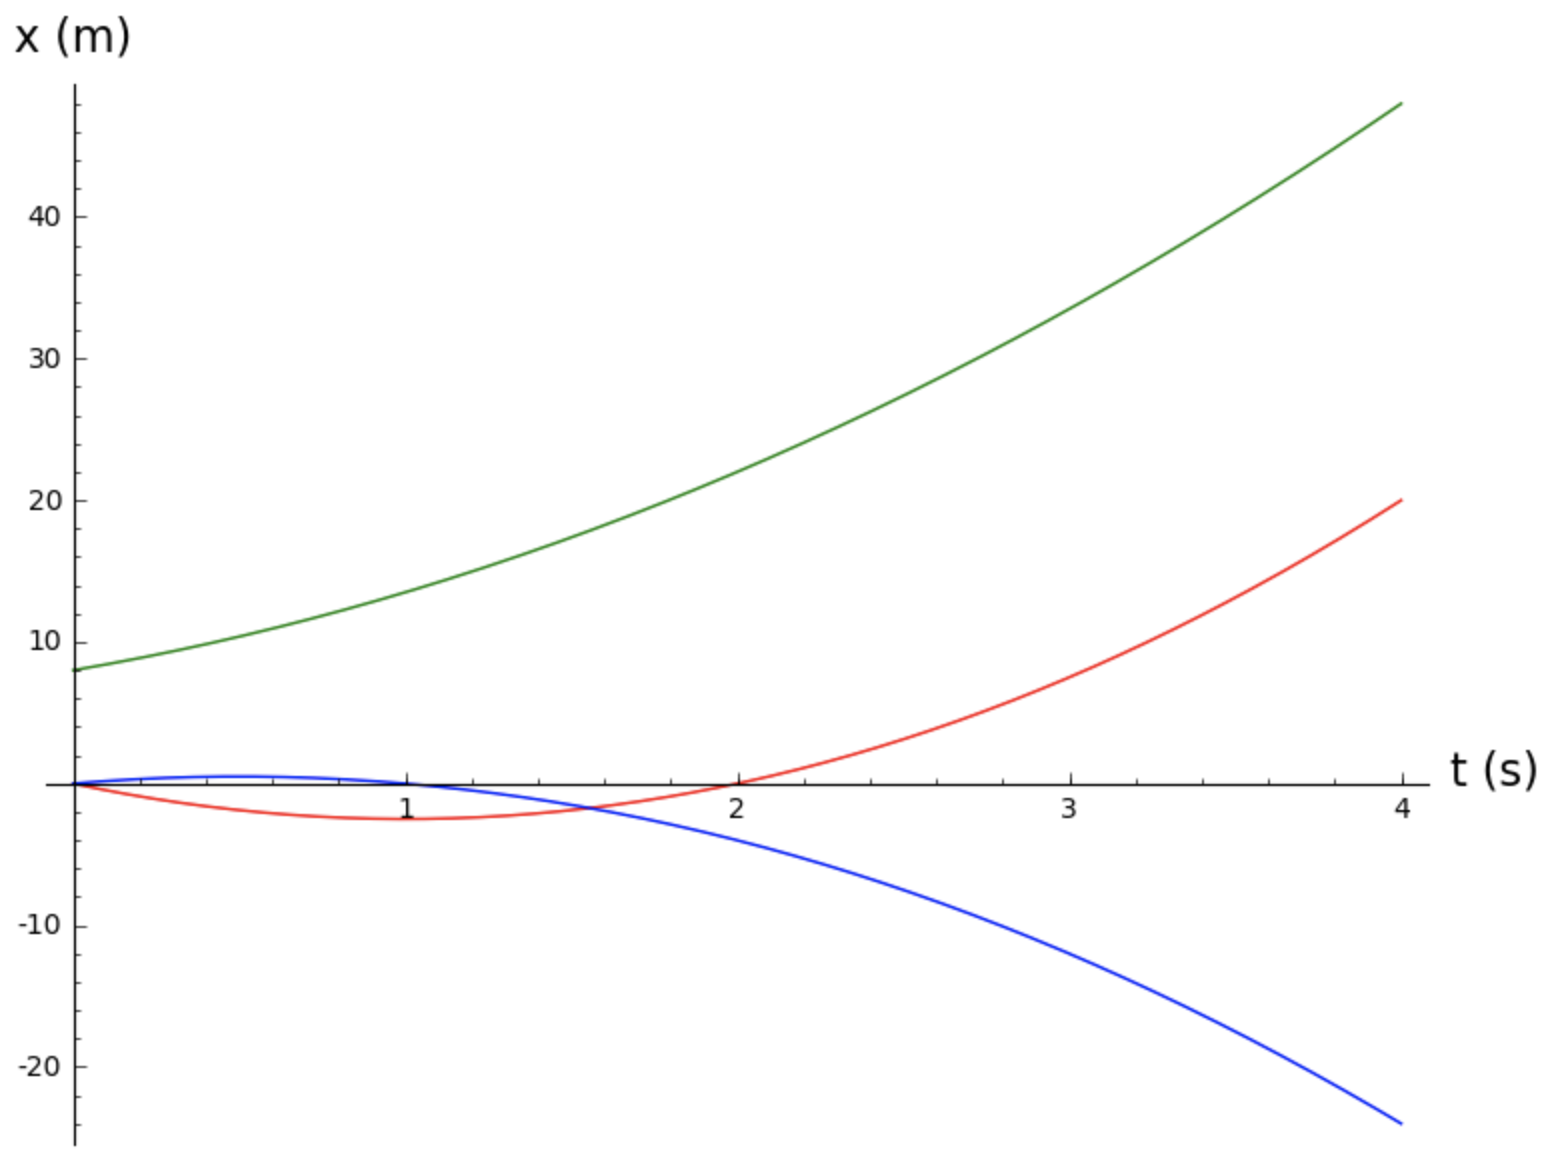
\includegraphics[scale=0.5]{threeCurves.png}

\underline{\textbf{Part 3}} \par
Now suppose you have some data collected from similar experiments on two other planets (different gravitational accelerations) (see planet1.txt and planet2.txt).
Use this data to determine
(a) the gravitational acceleration of each planet,
(b) the orientation of the axis used in the experiment (up or down),
(c) the magnitude and direction (up or down) of the initial velocity, and
(d) the starting coordinate of the ball.
Use the following approach:
\begin{enumerate}
\item Download manfit-app.zip from https://github.com/naharrison/manual-fitter/releases, unzip it, and open the jar file.
\item From the unzipped folder, also open data/XYdata.txt and data/fitFunction.txt. Try to understand how the data in these files is being used by the application.
\item Copy the data from planet[1,2].txt into XYdata.txt. Also modify fitFunction.txt to use a function that describes an object under constant acceleration: [0] + [1]*x + 0.5*[2]*x\string^2; the lines under the function are the minimum and maximum possible values for each parameter.
\item Restart the application and tune the parameters to determine the initial position, initial velocity, and acceleration.
\end{enumerate}


\end{document}
